\subsubsection{Bobusa-Gruppe}\label{sec:BBS-Gr}

Der Bobusa-Stil beschreibt eine nur unzureichend belegte keramische Ausprägung, die ausschließlich im äußersten Süden, an der Mündung des \mbox{Sangha} in den Kongo, erfasst wurde (Abb.~\ref{fig:BBS_Verbreitung}). Die Stücke zeichnen sich vornehmlich durch einfache Formen, sehr wenig Verzierungen und eine Magerung mit zerstoßener Keramik aus (Abb.~\ref{fig:BBS_Typverteter}). Keramik dieser Stilgruppe konnte an sechs Fundstellen geborgen werden. An neun weiteren Fundplätzen, vornehmlich entlang des \mbox{Sangha}, fanden sich vereinzelte GE, die unter Vorbehalt der Bobusa-Gruppe zugerechnet werden könnten. Die Gruppe setzt sich aus 125 individuell aufgenommenen GE sowie 73 ausgezählten Scherben zusammen. Über 53\,\% dieses Materials wurde jedoch nur unter Vorbehalt der Stilgruppe zuordnet. Über die Hälfte der Funde (56\,\%) stammt aus den beiden Grabungsbefunden BBS~87/1 sowie BBS~87/2 (Kat.-Nr.~6--7) am eponymen Fundort Bobusa (Fpl.~239). Während lediglich eine GE hinreichend erhalten war, um als Gefäß aufgenommen zu werden (Abb.~\ref{fig:BBS_Typverteter}.5), handelt es sich beim Großteil der Stücke um Fragmente von Gefäßwandungen (61\,\%). Randstücke machen 37\,\% des Inventars aus. In zwei Fällen konnten dedizierte Bodenstücke identifiziert werden (Taf.~33.16). Die aufgenommenen Stücke weisen eine sehr starke Fragmentierung auf, 87\,\% aller Stücke sind kleiner als 70\,$\times$\,70\,mm. Lediglich sieben GE waren zwischen 70\,$\times$\,70\,mm und 120\,$\times$\,120\,mm groß. Größere Fragmente wurden nicht beobachtet.

\begin{figure*}[tb]
	\begin{minipage}[b]{.8\textwidth}
		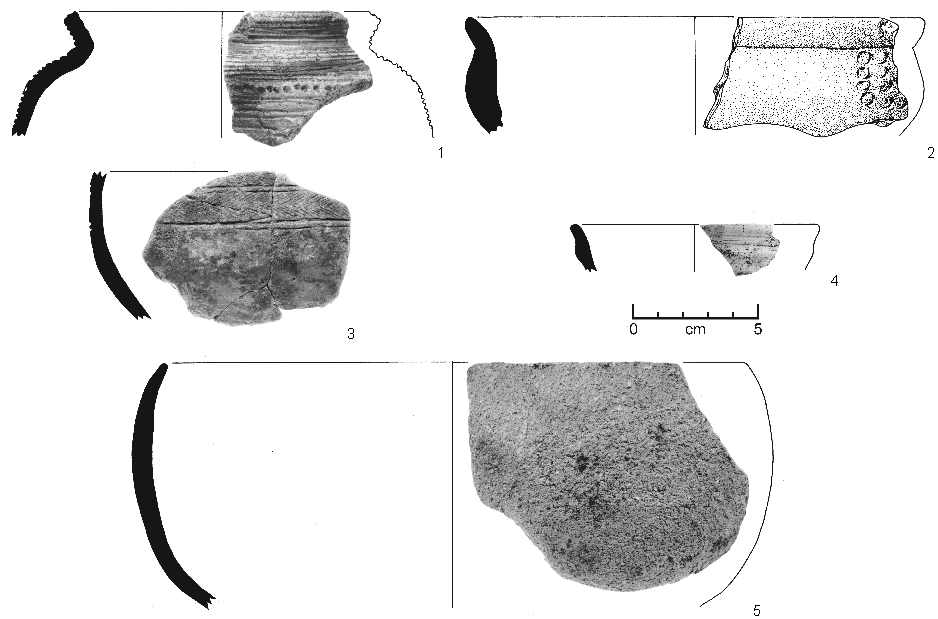
\includegraphics[width=\textwidth]{fig/BBS-Typen.pdf}
	\end{minipage}\hfill
	\begin{minipage}[b]{.2\textwidth}
		\caption{Bobusa-Gruppe: Typvertreter.\\1:~Taf.~33.10; 2:~Taf.~37.6; 3:~Taf.~33.12; 4:~Taf.~33.11; 5:~Taf.~33.5.}
		\label{fig:BBS_Typverteter}
	\end{minipage}
\end{figure*}

\paragraph{Technologische Merkmale}\hspace{-.5em}|\hspace{.5em}%
Die innerhalb der Bobusa-Gruppe subsumierte Keramik zeichnet sich mit Blick auf ihre technologischen Eigenschaften durch regelhaftes Vorkommen von Schamott -- zerstoßenen Keramikfragmenten -- im Scherben aus. Dieser als \textit{Fabric} 9 (Tab.~\ref{tab:Fabrics_Bilder}) systematisierte Zuschlag nichtplastischer Partikel macht 93\,\% der aufgenommenen GE aus. Alle übrigen GE enthalten neben Schamott auch weitere nichtplastische Bestandteile und sind dem \textit{Fabric} 8 zuordenbar. Die Anteile nichtplastischer Partikel im Scherben sind regelhaft sehr hoch, über 84\,\% aller Stücke weisen einen Anteil von mehr als 15--20\,\% auf. Nur sehr wenige Stücke zeigen geringere Anteile nichtplastischer Partikel. Die Partikel selbst sind vornehmlich den Größenklassen \textit{coarse} (43\,\%) sowie \textit{very coarse} (47\,\%) zuzuorden. Die Keramikfragmente, die dem Ausgangston künstlich beigemengt wurden, sind häufig bis auf eine Größe von knapp unterhalb 1\,mm zerkleinert worden und weisen regelhaft eine ausgeprägte Kantigkeit auf. Lediglich 18\,\% aller Stücke weisen eine Färbung auf, die auf die Nutzung eines rotbrennenden Tones hindeutet, während 24\,\% aufgrund ihrer grauen Färbung nicht näher angesprochen werden können. Ein großer Anteil (58\,\%) legt die Nutzung weißbrennender Tone nahe. Die Oberflächen der Scherben zeigen alle Zustände zwischen glatt (34\,\%), leicht rau (36\,\%) und rau (23\,\%), während die mittlere Dicke der Wandungen mit 8,5\,mm auffallend hoch ist.

\begin{figure*}[p]
	\centering
	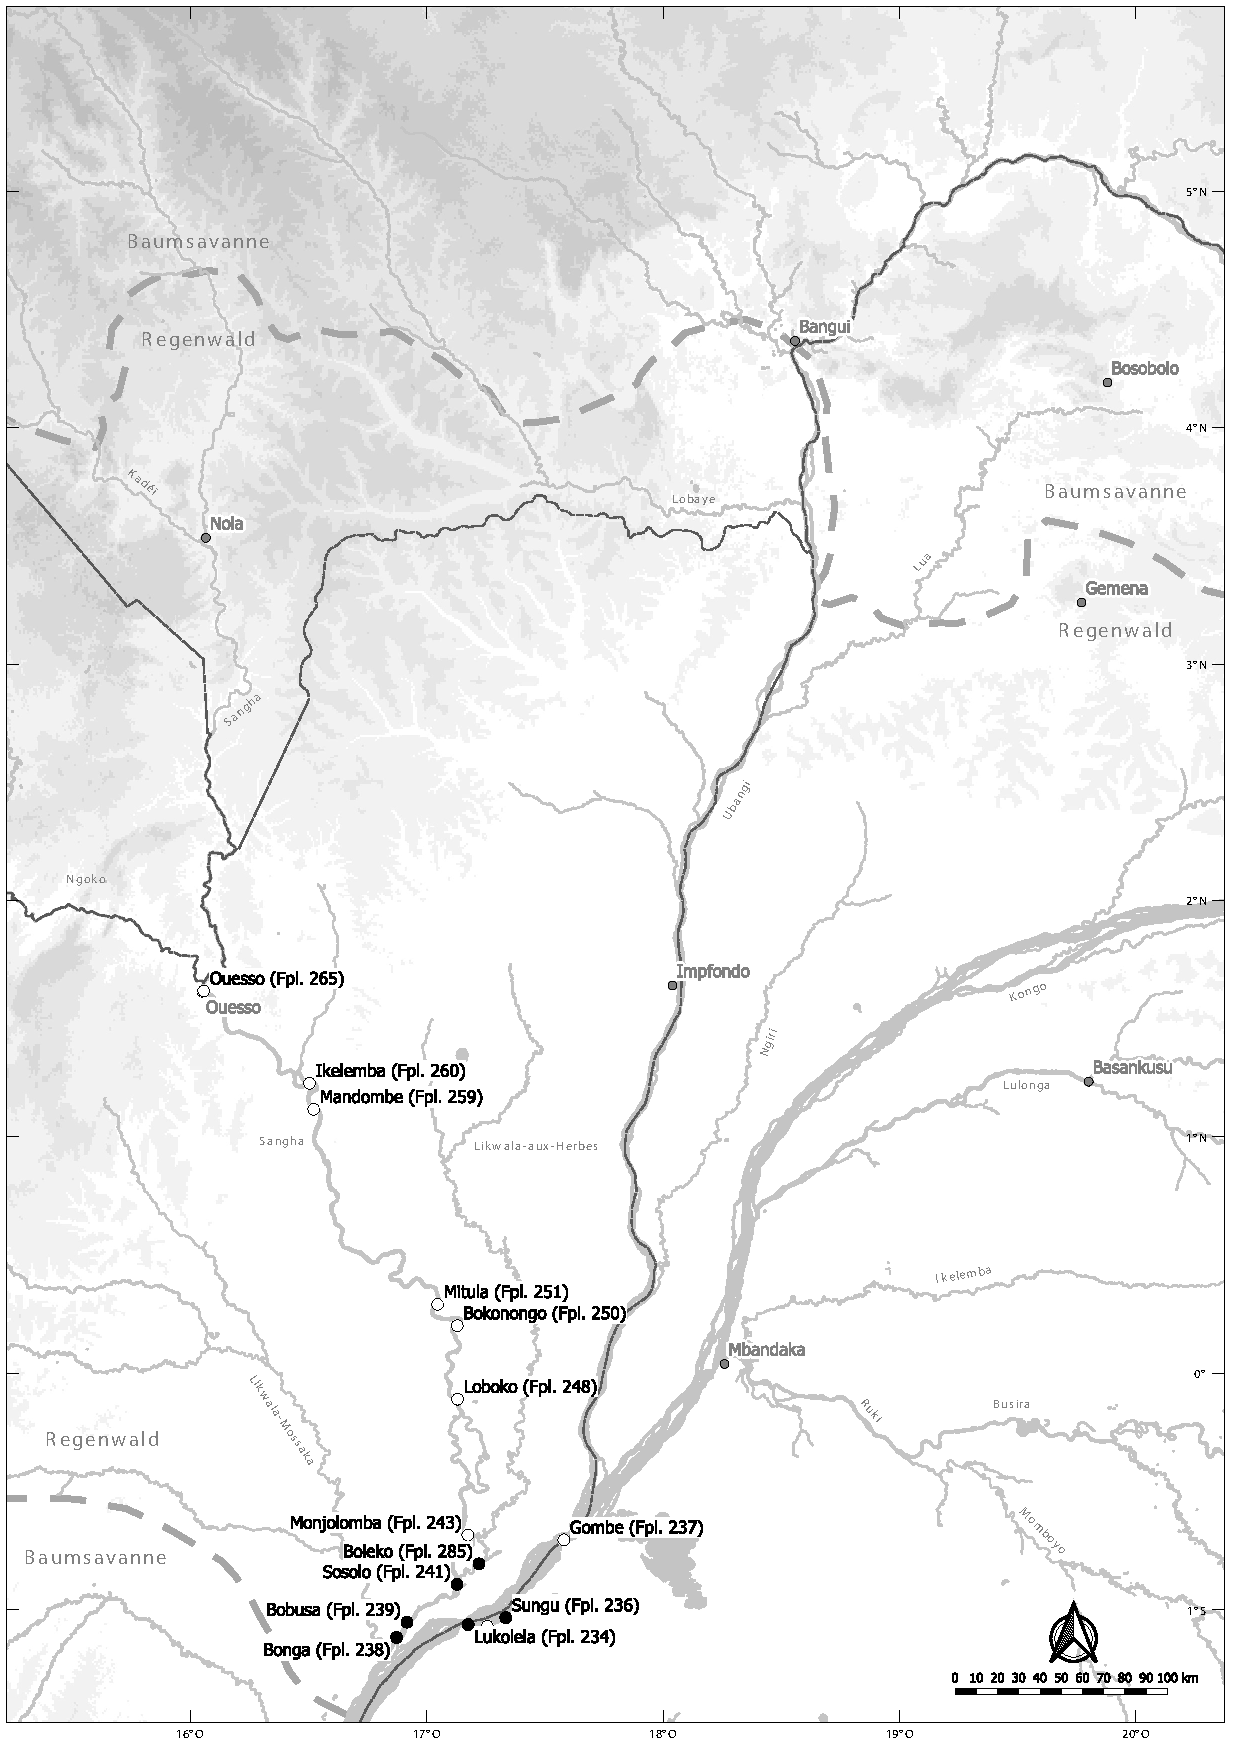
\includegraphics[width=\textwidth]{fig/BBS_Verbreitung.pdf}
	\caption{Bobusa-Gruppe: Verbreitung.}
	\label{fig:BBS_Verbreitung}
\end{figure*}

\paragraph{Formen}\hspace{-.5em}|\hspace{.5em}%
Die Gefäßform konnte lediglich bei 45~GE angesprochen werden und auch nur bei 24\,\% davon konnte die Zuweisung hinreichend sicher vorgenommen werden. Die starke Fragmentierung der Bobusa-Keramik sowie der große Anteil von Wandungsscherben im Inventar der Stilgruppe haben zur Folge, dass nur bedingt belastbare Aussagen zu den charakteristischen Gefäßformen gemacht werden können. Den größten Anteil der bestimmten Gefäßformen nehmen nicht näher spezifizierbare Gefäße mit geschweifter Wandung und ohne ausgeprägten Halsbereich ein (Typ~E; 38\,\%; Abb.~\ref{fig:BBS_Typverteter}.1). Schalenförmige Gefäße mit konvexer Wandung machen 24\,\% der aufgenommen Formen aus (Typ~I; Abb.~\ref{fig:BBS_Typverteter}.2,4) und schalenförmige Gefäße mit konvexer Wandung und einbiegendem Rand 18\,\% (Typ~H; Abb.~\ref{fig:BBS_Typverteter}.5). Die letztgenannte Form sowie die häufig beobachteten Gefäße mit geschweifter Wandung deuten eine grundsätzliche Ähnlichkeit der Inventare der Bobusa-Gruppe zu den Gefäßen von der Île des Mimosas (Kinshasa) an \parencite[siehe][279f.; Kap.~\ref{sec:Niederkongo}]{Eggert.1984}.\footnote{Die Grundform dieser Schalen lässt sich auch, sofern sie eine etwas elaboriertere Verzierung und keine Schamott-Magerung aufweist, innerhalb des Bokonongo-Stils finden (Kap.~\ref{sec:BOG-Gr}). Die Grabungen in Bobusa (Kat.-Nr. 6--7; Fpl.~239) erbrachten keine entsprechenden Formen. Erst zukünftige und intensivere Feldarbeiten in der Region werden eine Differenzierung zwischen den Gruppen ermöglichen.} Flaschenförmige Gefäße sowie Gefäße mit leicht konvexer Wandung und ausgeprägtem Halsbereich machen jeweils 7\,\% der Formen aus. Die maximalen Durchmesser der schalenförmigen Gefäße schwanken zwischen \mbox{16--26\,cm} und die der Gefäße mit geschweifter Wandung zwischen 11--31\,cm. Die Höhe der Mündung konnte lediglich bei einer GE hinreichend gut rekonstruiert werden (Abb.~\ref{fig:BBS_Typverteter}.5).\footnote{Die Schale mit einbiegendem Rand weist einen maximalen Durchmesser von 22,5\,cm auf und die Höhe liegt bei zirka 12\,cm. Daraus ergibt sich ein Höhen-Breiten-Verhältnis von zirka 2:1.} Bei 30~GE der Bobusa-Gruppe konnte die Randform bestimmt werden. Die Ränder sind regelhaft kurz und gerade ausbiegend (B1.1; 37\,\%) oder gerade ausbiegend mit einem innenseitigen Absatz (B1.5; 33\,\%).\footnote{Ausbiegende Ränder mit innenseitigem Grad vom Typ B1.5 sind vor allem von der rezenten Keramik der Mobaka-Gruppe bekannt (Kap.~\ref{sec:MKA-Gr}).} Die Randlippen sind häufig rund (46\,\%) oder spitz (35\,\%) ausgearbeitet. Lediglich bei drei GE der Bobusa-Gruppe konnte die Ausprägung des Gefäßbodens beobachtet werden. Während eine GE einen runden Boden vom Typ B1 aufweist, zeigt eine andere einen Flachboden mit konkaver Standfläche (B6) und die letzte einen Standringboden (B13).

\paragraph{Verzierung}\hspace{-.5em}|\hspace{.5em}%
Die Bobusa-Gruppe zeichnet sich durch eine starke Zurückhaltung von Dekor aus. Knapp über die Hälfte (55\,\%) aller GE weisen keine Verzierungen auf. Die verzierten Stücke zeigen häufig lediglich ein bis zwei Verzierungselemente. Am häufigsten lassen sich in Ritztechnik produzierte Riefen- und Rillen beobachten (Tab.~\ref{tab:Verzierungselemente}: 01--02). Diese machen 74\,\% aller aufgenommenen Verzierungselemente aus, wobei allein 58\,\% aller Verzierungen horizontale Rillen sind (Tab.~\ref{tab:Verzierungselemente}: 02.1). Sie finden sich mit Ausnahme des Bodenansatzes sowie der Standfläche auf nahezu allen Positionen am Gefäß (Anlage~4\subref{fig:BBS_Verz}). Das Gros der Verzierungen findet sich im Bauchbereich der Gefäße (36\,\%) sowie dem Rand (20\,\%). Neben den horizontalen Rillen treten deutlich seltener \textit{Schachbrett}-Muster aus diagonalen Rillen (Tab.~\ref{tab:Verzierungselemente}: 01.2; 7\,\%) sowie horizontale Reihen aus diagonal gestellten Eindrücken auf (Tab.~\ref{tab:Verzierungselemente}: 04.2; 3\,\%). Eine charakteristische Eigenheit der Bobusa-Keramik ist das Vorkommen von Resten roter Bemalung (Tab.~\ref{tab:Verzierungselemente}: 14.2; 6\,\%). Diese findet sich ebenfalls an allen Gefäßpartien mit Ausnahme der unteren Hälften sowie des Randes. Reste von roter Bemalung finden sich ausschließlich als horizontale Streifen, häufig in den Vertiefungen von Rillen und Riefen.\footnote{Siehe auch entsprechende Exemplare von rezent genutzten mobilen, für die Nutzung auf Reisen in Einbäumen vorgesehenen Herden mit roter Bemalung in Kap.~\ref{sec:Reiseherde}.}

\paragraph{Datierung}\hspace{-.5em}|\hspace{.5em}%
Für die Datierungen des Bobusa-Stils liegen aus dem Arbeitsgebiet keine absoluten Daten vor. Sie lässt sich mit Blick auf Morphologie, Ornamentik und \textit{Fabric} nur vage an andere Stilgruppen des Arbeitesgebiets sowie des benachbarten Inneren Kongobeckens anbinden. Die aktuell besten Vergleiche bieten Funde aus der Region um Kinshasa, genauer von der Île des Mimosas (siehe \textsc{Eggert} 1984a: 279\,f.). Ein Radiokohlenstoffdatum stellt die bislang nicht vollständig veröffentlichten Funde dieser Fundstelle in das 2.--4.~Jh. n.~Chr. (siehe Kap.~\ref{sec:Niederkongo}). Auf Basis dieses Vergleichs wird für die entsprechende Keramik des Bobusa-Stils eine provisorische Datierung in das 2.--4.~Jh n.~Chr. vorgeschlagen.

\paragraph{Verbreitung}\hspace{-.5em}|\hspace{.5em}%
Keramik der Bobusa-Gruppe findet sich ausschließlich an sechs Fundplätzen in einem eng begrenzten Gebiet im Bereich der Mündung des \mbox{Sangha}, im äußersten Süden des Arbeitsgebietes (Abb.~\ref{fig:BBS_Verbreitung}). Der südlichste Fundplatz ist Bonga (Fpl.~238) an der Mündung des \mbox{Sangha} in den Kongo, der nördlichste Boleko (Fpl.~185) am unteren Likwala-aux-Herbes. Das Verbreitungsgebiet sicher der Bobusa-Gruppe zuweisbarer Stücke -- innerhalb des Arbeitsgebietes -- erstreckt sich lediglich auf knapp 35\,km in Nord--Süd- sowie etwa 50\,km in Ost--West-Richtung. Es kann als sehr wahrscheinlich gelten, dass weiter stromabwärts des Kongo-Stroms weitere Funde dieser Stilgruppe gemacht werden können und die südliche Grenze der Verbreitung aktuell lediglich die Grenze des Arbeitsgebietes nachzeichnet. Unter Vorbehalt der Bobusa-Gruppe zuweisbare Stücke fanden sich als Einzelfunde entlang fast des gesamten befahrenen Abschnitts des \mbox{Sangha}. Den nördlichsten Fundpunkt dieses erweiterten Verbreitungsgebietes bildet die Fundstelle Ouesso (Fpl.~265) an der Grenze zu Kamerun, knapp 300\,km nordnordwestlich des Hauptverbreitungsgebietes.